\chapter{Variables}
{ }\hfill\textbf{Level:} Newbie\\ \\
\noindent Sometimes, it's necessary to draw a figure on a different scale. For example, if we want to draw a square with side length 100, a square with side length 200 and a square with side length 50, we need actually three different procedures  for each square.
\begin{verbatim}
to square1
repeat 4 [forward 100 right 90]
end
to square2
repeat 4 [forward 200 right 90]
end
to square3
repeat 4 [forward 50 right 90]
end
\end{verbatim}
We can see immediately that it would be easier to define a single procedure waiting for an argument: the side length. For example, \texttt{square 200} should draw a square with side length 200, \texttt{square 100} should draw a square with side length 100 ... It's time to introduce the variable notion!
\section{Examples}
\noindent To draw a square with side length 100, we write in the editor:
\begin{verbatim}
to square
repeat 4 [forward 100 right 90]
end
\end{verbatim}  
We just have to modify this procedure by doing:
\begin{itemize}
 \item We add \texttt{:c} at the end of the definition line. This indicates that the procedure is now waiting for an argument called \texttt{:c}
 \item We replace the side length 100 by the variable name \texttt{:c}
\end{itemize}
We obtain
\begin{verbatim}
to square :c
repeat 4 [forward :c right 90]
end
\end{verbatim}
Therefore, if we write: \texttt{square 100 square 50 square 30 square 20 square 10}\\
 \begin{center}
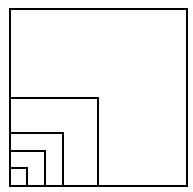
\includegraphics[scale=0.5]{pics/variables-carres.png}
\end{center}
 \vspace{1cm}
 \section{Drawing a rectangle with chosen dimension}
 \noindent We define here a procedure called \texttt{rec} depending on two variables representing the dimensions of the rectangle. Hence \texttt{rec 200 100} will draw a rectangle with height 200 and width 100.
 \begin{verbatim}
to rec :lo :la
repeat 2 [forward :lo right 90 forward :la right 90]
end
\end{verbatim} 
Make some examples: 
\begin{verbatim}
rec 200 100 rec 100 300 rec 50 150 rec 1 20 rec 100 2 
\end{verbatim}
If we give to the procedure \texttt{rec} only one number, the interpreter will send an error message indicating that the procedure is waiting for a second argument.
\section{Drawing at different scales}
\noindent We saw how to draw a square, and a rectangle with different sides. Now, we return to our house example p. \pageref{maison} and we're going to modify the code to draw this house at any chosen scale.\\ \\
The objective is to send an argument to the procedure \texttt{house} and according to this parameter, the house will be smaller or bigger. 
\begin{itemize}
 \item \texttt{house 1} will draw the house in real size.
 \item \texttt{house 0.5} will draw the house at scale 0.5.
 \item \texttt{house 2} will draw the house with double proportion.
\end{itemize}
In real size, the procedure square was:
\begin{verbatim}
to square
repeat 4 [forward 150 right 90]
end
\end{verbatim}
All the initial dimensions are multiplied by the scale. Hence, the procedure \texttt{square} becomes: 
\begin{verbatim}
to square :c
repeat 4 [forward 150*:c right 90]
end
\end{verbatim}
Therefore, when we'll write \texttt{square 2}, the square will have for side length $150\times2=300$. Proportions are well respected! In fact, we can see that we just need to modify all procedures replacing the length according to this rule: \\
\texttt{fd 70} becomes \texttt{fd 70*:c} \\
\texttt{fd 45} becomes \texttt{fd 45*:c} \\  
\begin{verbatim}
to carre :c
repeat 4[forward 150*:c  right 90]
end

to tri :c
repeat 3[forward 150*:c right 120]
end

to porte :c
repeat 2[forward 70*:c right 90 forward 50*:c right 90]
end

to che :c
forward 55*:c right 90 forward 20*:c right 90 forward 20*:c
end

to dep1 :c
right 90 forward 50*:c left 90
end

to dep2 :c
left 90 forward 50*:c right 90 forward 150*:c right 30
end

to dep3 :c
penup right 60 forward 20*:c left 90 forward 35*:c pendown
end

to ma :c
carre :c dep1 :c porte :c dep2 :c tri :c dep3 :c che :c
end
\end{verbatim}
\section{Exercice:}
\noindent Try to generate the following drawings at different scales.\\ \\ \\
\begin{center}
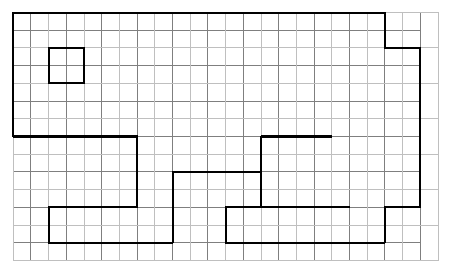
\includegraphics[scale=0.6]{pics/variables-grenouille.png}
\end{center}
\begin{center}
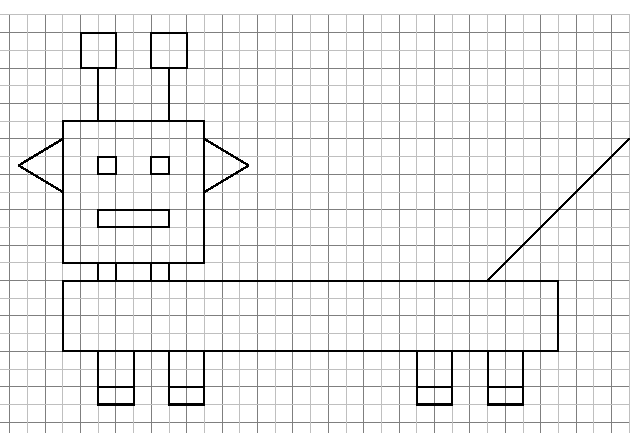
\includegraphics[scale=0.75]{pics/variables-robot.png}
\end{center}
